 %\documentclass[handout]{beamer}
\documentclass{beamer}

\usepackage{subfigure}
\usepackage{graphicx}
\usepackage{sidecap}
\usepackage{caption}
%\usepackage{subcaption}
%\captionsetup{compatibility=false}
\usepackage{appendixnumberbeamer}
\usepackage{amsmath}
% --
\usepackage{multirow}
\usepackage{xcolor}
\usepackage{setspace}
\usepackage{hyperref}
\usepackage{anyfontsize}
\usepackage{array, makecell} %

\setbeamertemplate{footline}

\newenvironment{itemise} {\begin{itemize} \setlength{\itemsep}{0.2cm}} {\end{itemize}}
%\usepackage[labelformat=empty]{caption}
\setbeamertemplate{sections/subsections in toc}[square]

%% COLORS
\definecolor{Gray}{gray}{0.9}
\definecolor{dblue}{rgb}{0.132,0.1,0.27}
\definecolor{mint}{cmyk}{1.0, 0.2, 0.6, 0.05}
\definecolor{ant}{cmyk}{0.5, 0.1, 0.0, 0.45}
\definecolor{lgray}{cmyk}{0.12, 0.0, 0.0, 0.17}
\definecolor{lred}{cmyk}{0.0, 0.9, 0.7, 0.0}

%\setlength{\leftmargini}{0pt}


\usepackage{etoolbox}% http://ctan.org/pkg/etoolbox 
\usepackage{booktabs}

\newenvironment{literatur}{%
  \parskip1pt \parindent0pt \raggedright
  \def\lititem{\hangindent=0.3cm \hangafter1}}{%
  \par\ignorespaces}

\newcommand{\tb}[1]{{\color{dblue}{\textbf{#1}}}}
\newcommand{\tm}[1]{{\color{mint}{\textbf{#1}}}}
\newcommand{\tr}[1]{{\color{lred}{\textit{#1}}}}

%\href{<Ziel>}{<Eingefasster Text>} 

%\logo{\includegraphics[height=0.7cm]{BdFlogo.eps}\hspace{300pt}\vspace{-5pt}}
%\logo{\includegraphics[height=0.8cm]{BdFlogo.eps}}
%\logo{\pgfputat{\pgfxy(-6.2,-0.5)}{\pgfbox[center,base]{\includegraphics[height=0.8cm]{BdFlogo.eps}}}}


%------------------------------------------------------------------------------------
% TITLE
%------------------------------------------------------------------------------------
\title[PSME]{Macroeconomics\\ - Lecture 7 -}
\author[Grosse Steffen]{Christoph Gro{\ss}e Steffen}
\institute[BdF]{PSME Panth\'{e}on-Sorbonne Master in Economics}
\date[PSME macro]{3 November 2021}

%---BEGIN------------------------------------------------------------------------------
\begin{document}
%---BEGIN------------------------------------------------------------------------------
\begin{frame}
\maketitle
\end{frame}
%---FRAME------------------------------------------------------------------------------
%\section{Outline}
\begin{frame}
\frametitle{Outline}
\begin{center}
\tb{(7) Nominal rigidities}
\end{center}

\tableofcontents
\end{frame}
%---FRAME------------------------------------------------------------------------------
\section{Micro evidence}
%---FRAME------------------------------------------------------------------------------

%---FRAME------------------------------------------------------------------------------
\begin{frame}{Nominal rigidities}

Central \tb{Keynesian assumption:} Prices do not adjust immediately \\
($\rightarrow$ \alert{sticky prices} = slow moving)

\begin{itemize}
\small
\item Make things simpler: assume \tb{prices are fixed in the short-run}.
\item $\Rightarrow$ Interaction between nominal and real side of the economy!
\item As a result, \tb{disturbances} in goods and financial markets give rise to \emph{business cycle fluctuations}.
\item In contradiction with the \tm{money neutrality principle} (\tb{long-run!})
\end{itemize}

\emph{How reasonable is this assumption?}
\begin{itemize}
\small
\item Answer: It is a good approximation
\item This lecture with detailed empirical results.
\end{itemize}

\end{frame}

%---FRAME------------------------------------------------------------------------------
\begin{frame}{Micro evidence on price-setting}

\begin{center}
\emph{Are prices flexible or sticky?}
\end{center}

\begin{itemize}
%\small
%\item Question at the center of explaning business cycles
%\item also divides Keynesian and classical views
\item This lecture: \tb{empirical approach}
\begin{itemize}
\small
\item Review empirical micro price studies
\item What is the role of price seeting for business cycles?
\end{itemize}
\end{itemize}

{\scriptsize
based on: Klenow, P.J. and Malin, B.A. (2011) "Microeconomic evidence on price-setting", \emph{Handbook of Monetary Economics}, Vol. 3A, 231-284.
}
\end{frame}

%---FRAME------------------------------------------------------------------------------
\subsection{Data and average frequency of price changes}
\begin{frame}
\frametitle{Outline}
\tableofcontents[currentsubsection]
\end{frame}
%---FRAME------------------------------------------------------------------------------
\begin{frame}{Price rigidity: data}

\begin{itemize}
\small
\item Evidence from the euro area points to sticky pices
\end{itemize}

\begin{center}
%{\small
%Figure. Liability = a promise to payout the holder of the note  \\
%}

%\vspace{-2mm}
\begin{figure}[h!]
%\caption{Figure. Capital share US, 1946-2018
	%\subfigure{\includegraphics<1>[trim=80 60 100 70,clip,width=0.75\textwidth]{FIGURES/3_Autarky}
	%}
	\subfigure{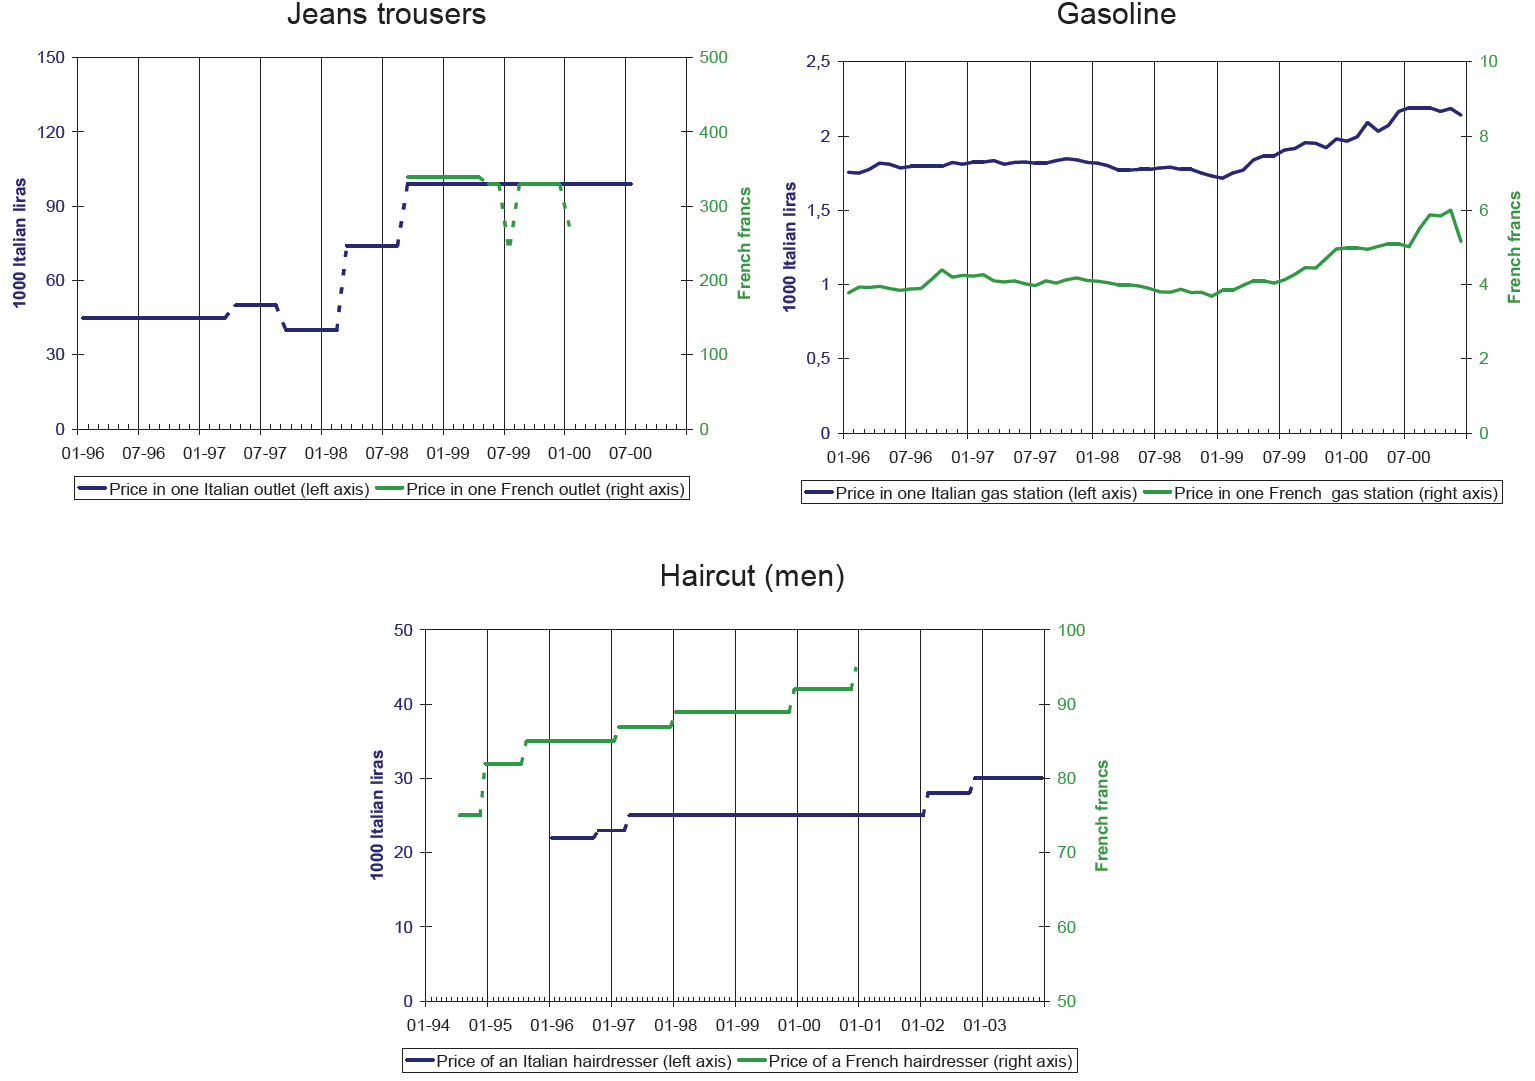
\includegraphics[trim=0 0 0 0,clip,width=0.8\textwidth]{FIGURES/6_PriceChangesEA}
	}      
	%\subfigure{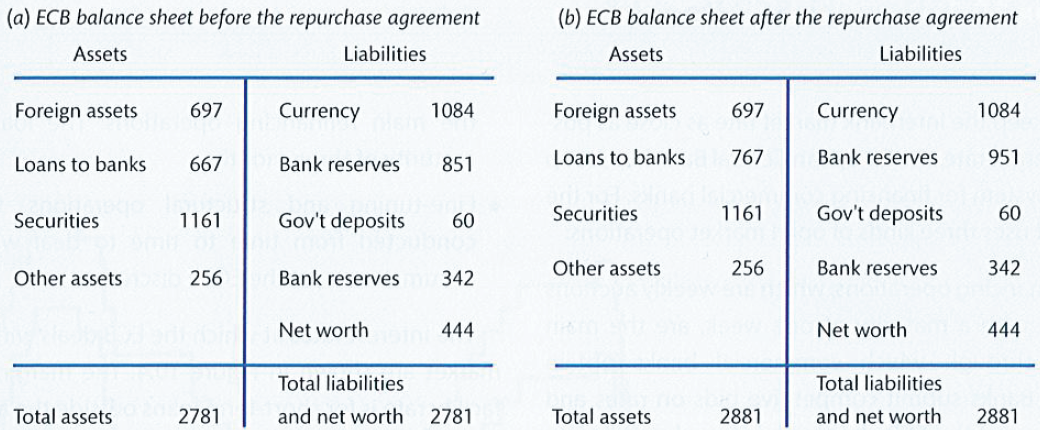
\includegraphics[trim=0 00 0 00,clip,width=0.6\textwidth]{FIGURES/5_CB_balance_sheet_OMO}
	%} 
	
%	\label{fig:GPD} 
	%[trim=left bottom right top
\end{figure}
%\vspace{-2mm}

\begin{minipage}{1.0\columnwidth}
\tiny	
\textbf{Note.} Actual examples of trajectories, extracted from the French and Italian CPI databases. The dotted lines indicate events of price changes.
\textbf{Source.} Dhyne et al (2005) 'Price setting in the euro area: Some stylized facts from individual consumer price data', Figure 1.\\
\end{minipage}
\end{center}

\end{frame}
%---FRAME------------------------------------------------------------------------------
\begin{frame}{What can we learn from micro price data?}

\begin{itemize}
\small
\item How often do prices change?
\item Do price changes 'cancel out' after aggregation?
\begin{itemize}
\small
\item cross-sectional aggregation
\item aggregation over time
\end{itemize}
\item Do prices respond to aggregate (macro) shocks?
\end{itemize}

$\rightarrow$ important implications for models
\end{frame}
%---FRAME------------------------------------------------------------------------------
\begin{frame}{Data sources}

\begin{enumerate}
\item Data underlying the construction of \tb{price indices}, such as the consumer price indices (CPI), or producer prices indices (PPI)
\item \tb{Scanner and online prices}, directly from retailers
\item \tb{Surveys} of price setters
\end{enumerate}

\end{frame}
%---FRAME------------------------------------------------------------------------------
\begin{frame}{1. Data underlying price indices}

\begin{itemize}
\small
\item Data underlying the construction of price indices, such as the consumer price indices (CPI), or producer prices indices (PPI)
\begin{itemize}
\small 
\item National statistical agencies collect monthly price quotes
\item Representative (products, geography, outlet, ...)
\item US: $>85.000$ price quotes per month (Bureau of Labor Statistics)
\end{itemize}
\item Results (Table 1)
\begin{itemize}
\small
\item median of average frequency of price changes is \tb{19\% per month}
\item empirical \tb{evidence for price stickiness}
\item substantial \tb{cross-country heterogeneity} (US vs. Euro area/ AEs vs EMEs)
\end{itemize}
\end{itemize}

\end{frame}
%---FRAME------------------------------------------------------------------------------
\begin{frame}

\begin{center}

\begin{figure}[h!]
	\subfigure{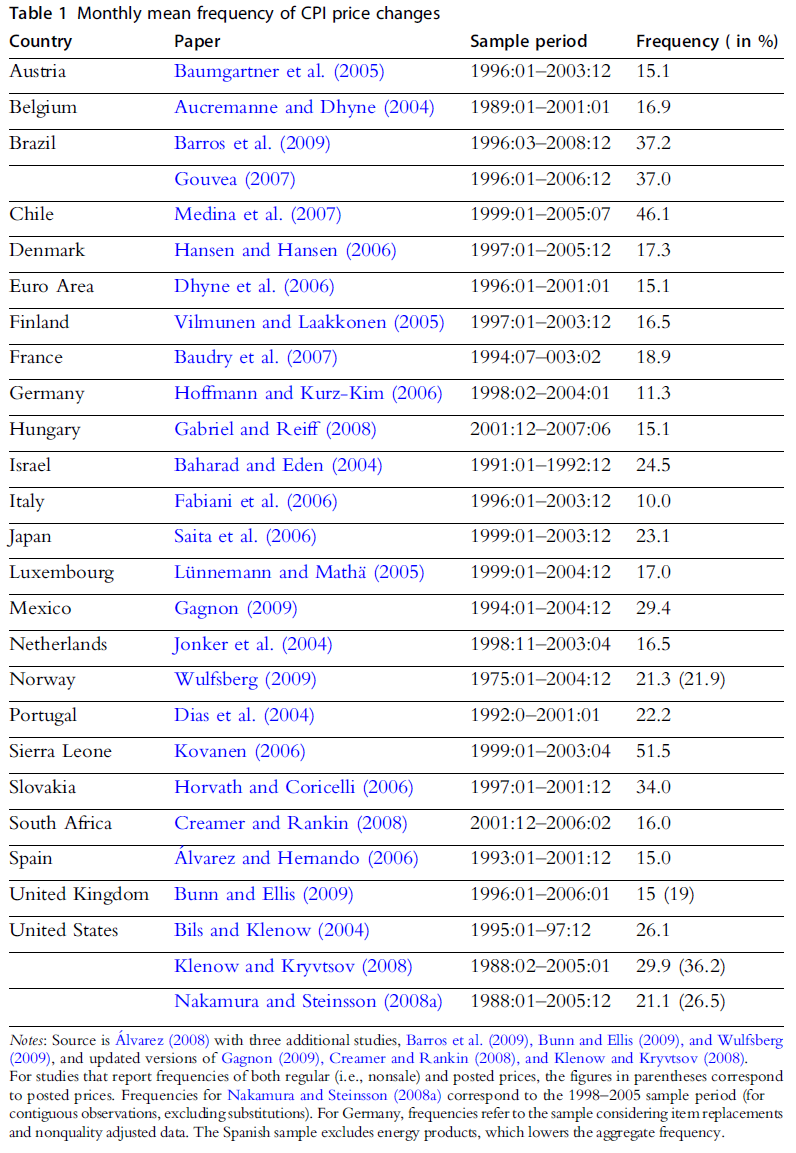
\includegraphics[trim=0 0 0 0,clip,width=0.7\textwidth]{FIGURES/PriceSetting/Table1_cpiPriceChanges}
	}      

\end{figure}
%\vspace{-2mm}

%\begin{minipage}{0.6\columnwidth}
%\tiny	
%%\textbf{Note.}
%\end{minipage}
\end{center}


\end{frame}
%---FRAME------------------------------------------------------------------------------
\begin{frame}{Distribution of frequency of price changes}


\begin{itemize}
\small
\item BLS collects prices of 300 categories (Entry Level Items/ELIs) of consumer goods and services
\item median $<$ mean (frequency of price changes) due to convex distribution
\end{itemize}

\begin{center}

\begin{figure}[h!]
	\subfigure{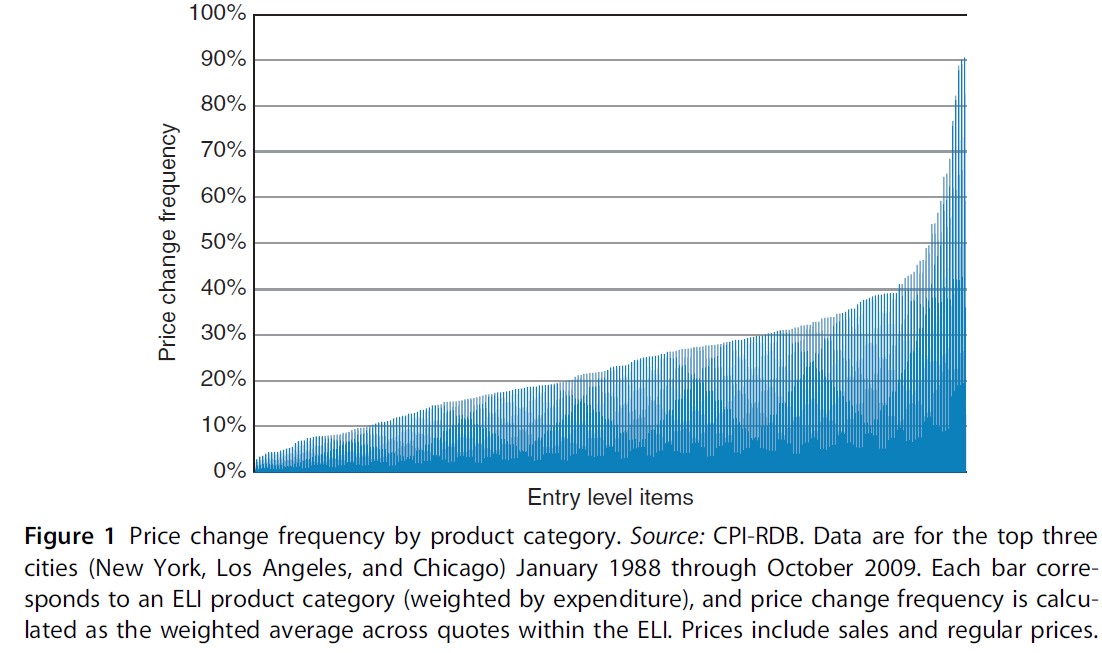
\includegraphics[trim=0 0 0 0,clip,width=0.7\textwidth]{FIGURES/PriceSetting/Fig1_distrFrequencyPriceChanges}
	}      
\end{figure}
%\vspace{-2mm}

%\begin{minipage}{0.6\columnwidth}
%\tiny	
%%\textbf{Note.}
%\end{minipage}
\end{center}

\begin{itemize}
\scriptsize
\item 2.7\% 'Intracity Mass Transit' -vs- 91\% 'Regular Unleaded Gasoline'
\end{itemize}

\end{frame}
%---FRAME------------------------------------------------------------------------------
\begin{frame}{2. Scanner data}


\begin{itemize}
\small
\item Scanner and online prices, directly from retailers
\begin{itemize}
\small
\item what do 'on-the-shelf' prices measure? (\emph{call options with unlimited quantities?'})
\item difficult to assess other price-determining variables (quality margins, buyer characteristics)
\end{itemize}
\end{itemize}

\end{frame}
%---FRAME------------------------------------------------------------------------------
\begin{frame}


\begin{center}
%\vspace{-2mm}
\begin{figure}[h!]
	\subfigure{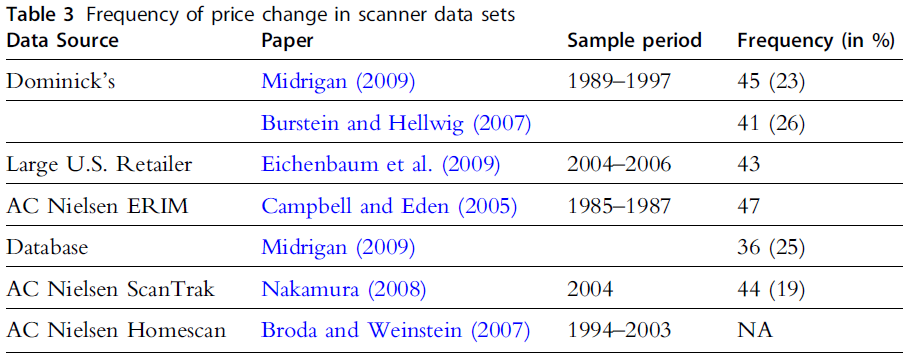
\includegraphics[trim=0 0 0 0,clip,width=0.9\textwidth]{FIGURES/PriceSetting/Table3_scannerData}
	}      
\end{figure}
%\vspace{-2mm}

%\begin{minipage}{0.6\columnwidth}
%\tiny	
%%\textbf{Note.} 
%\end{minipage}
\end{center}

\end{frame}
%---FRAME------------------------------------------------------------------------------
\begin{frame}{3. Surveys of price setters}

\begin{itemize}
\small
\item Ask firms directly how often they changed prices
\item ...also ask them how often they \emph{review} their prices
\end{itemize}



\end{frame}
%---FRAME------------------------------------------------------------------------------
\begin{frame}

\begin{center}

\begin{figure}[h!]
	\subfigure{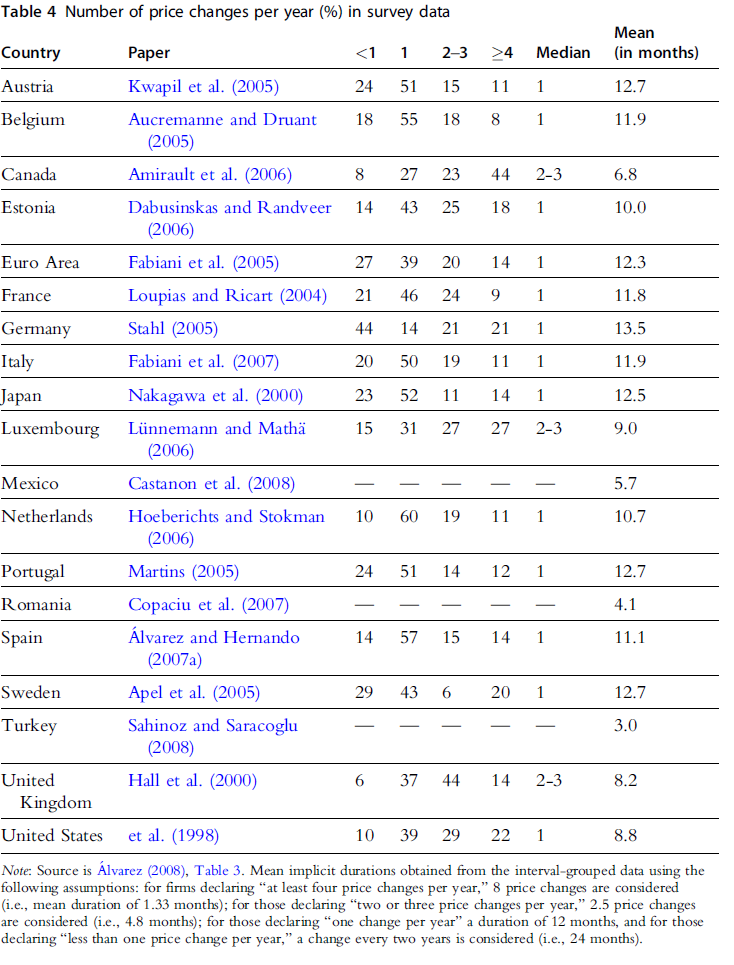
\includegraphics[trim=0 0 0 0,clip,width=0.7\textwidth]{FIGURES/PriceSetting/Table4_surveyData}
	}      

\end{figure}
%\vspace{-2mm}

%\begin{minipage}{0.6\columnwidth}
%\tiny	
%%\textbf{Note.}
%\end{minipage}
\end{center}

\end{frame}
%---FRAME------------------------------------------------------------------------------
\begin{frame}{Some remarks on 'average' frequency of price changes}

\begin{itemize}
\small
\item \tb{results across studies can differ}, even when using the same data set
\begin{itemize}
\small
\item methodological differences (e.g. mean frequency for one store -vs- mean frequency per product category)
\item sample periods, coverage
\end{itemize}
\item despite differences: \tb{prices change at least once per year}
\end{itemize}


\end{frame}
%---FRAME------------------------------------------------------------------------------
\subsection{Heterogeneity}
\begin{frame}
\frametitle{Outline}
\tableofcontents[currentsubsection]
\end{frame}
%---FRAME------------------------------------------------------------------------------
\begin{frame}{Heterogeneity: Frequency -vs- durability of goods}


\begin{itemize}
\small
\item Examples:
\begin{itemize}
\item $Transportation=durable+flexible$
\item $Food=nondurable+flexible$
\end{itemize}
\item No correlation between frequency of price changes and durability of the good
\item but strong positive correlation if remove raw goods (fresh food and energy) 
\end{itemize}


\begin{center}

\begin{figure}[h!]
	\subfigure{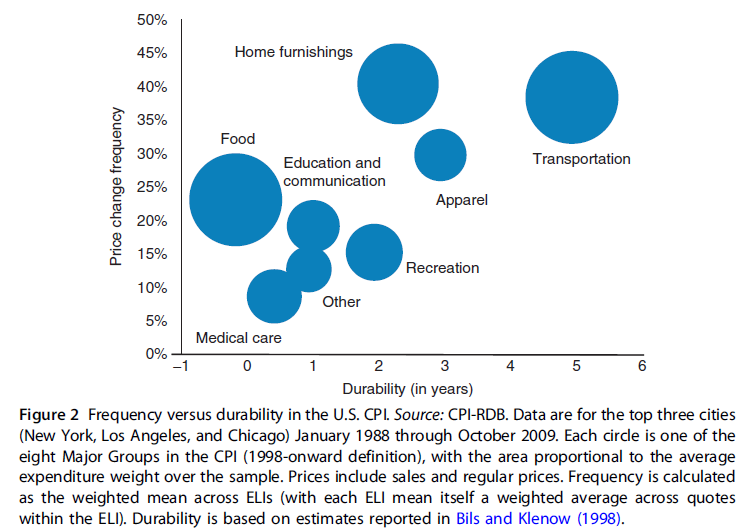
\includegraphics[trim=0 0 0 0,clip,width=0.7\textwidth]{FIGURES/PriceSetting/Fig2_frequencyDurability}
	}      

\end{figure}
%\vspace{-2mm}

%\begin{minipage}{0.6\columnwidth}
%\tiny	
%%\textbf{Note.}
%\end{minipage}
\end{center}


\end{frame}
%---FRAME------------------------------------------------------------------------------
\begin{frame}{Heterogeneity: frequency and cyclicality}

\begin{itemize}
\small
\item Product items with demand highly sensitive to the business cycle exhibit higher frequency of price changes!
\item Causality runs in both directions ($frequency \leftrightarrow cyclicality$)
\begin{itemize}
\item frequency $\rightarrow$ cyclicality: amplification of aggregate (supply) shocks in the presence of higher frequency of adjusting prices
\item cyclicality $\rightarrow$ frequency: more cyclical sectors face higher demand elasticities
\end{itemize}
\end{itemize}

\begin{center}

\begin{figure}[h!]
	\subfigure{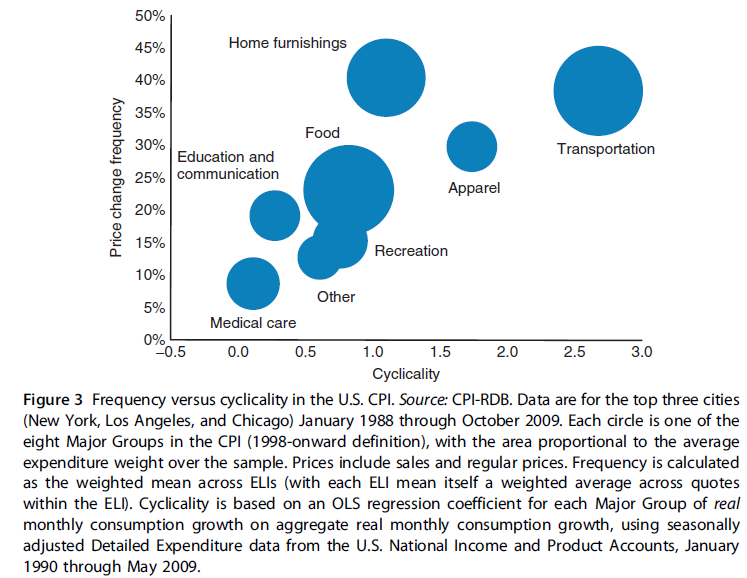
\includegraphics[trim=0 0 0 0,clip,width=0.7\textwidth]{FIGURES/PriceSetting/Fig3_frequencyCyclicality}
	}      

\end{figure}
%\vspace{-2mm}

%\begin{minipage}{0.6\columnwidth}
%\tiny	
%%\textbf{Note.}
%\end{minipage}
\end{center}

\end{frame}

%---FRAME------------------------------------------------------------------------------
\begin{frame}{Heterogeneity: frequency and inflation level}

\begin{itemize}
\small
\item Cross-country differences in frequency of price changes
\item Figure suggests that this might be due to higher average inflation
\begin{itemize}
\small
\item ...but higher inflation also more volatile in practice. So, correlation might be driven by level and variability
\item Insignificant findings: Dhyne et al. 2006
\end{itemize}
\end{itemize}

\begin{center}

\begin{figure}[h!]
	\subfigure{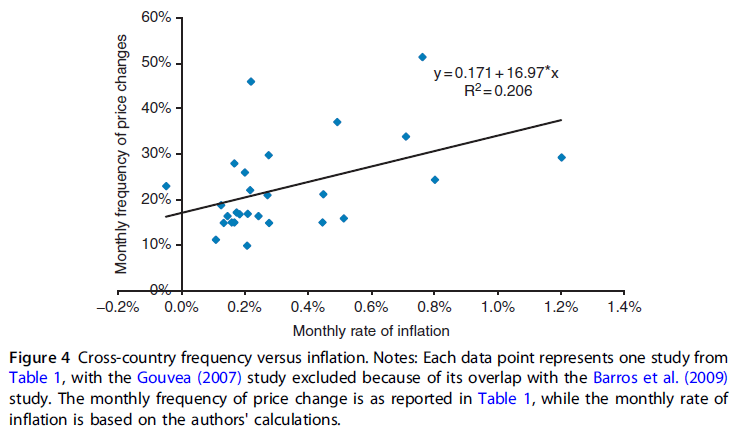
\includegraphics[trim=0 0 0 0,clip,width=0.7\textwidth]{FIGURES/PriceSetting/Fig4_frequencyInflation}
	}      

\end{figure}
%\vspace{-2mm}

%\begin{minipage}{0.6\columnwidth}
%\tiny	
%%\textbf{Note.}
%\end{minipage}
\end{center}

\end{frame}
%---FRAME------------------------------------------------------------------------------
\subsection{The role of sales prices}
%---FRAME------------------------------------------------------------------------------
\begin{frame}{The role of sales prices}

\begin{itemize}
\small
\item What is the role of sales on the frequency of price changes?
\item Sales, or transitory price changes, might have very different macroeconomic implications
\item \tb{Approach:} split prices into categories (\emph{reference, novel, comeback})
\end{itemize}

\end{frame}
%---FRAME------------------------------------------------------------------------------
\begin{frame}{Reference prices}

\begin{itemize}
\small
\item Price quotes are clustered: many prices are recurrent
\item Eichenbaum et al. 2009 define a sticky \tb{reference price} as the \tb{modal price}, i.e. the most quoted price, in each quarter.
\item Reference prices are more persistent (prices change every 11.1 months instead of 3 months)
\end{itemize}

\end{frame}
%---FRAME------------------------------------------------------------------------------
\begin{frame}{Reference prices}

\begin{center}
\begin{figure}[h!]
	\subfigure{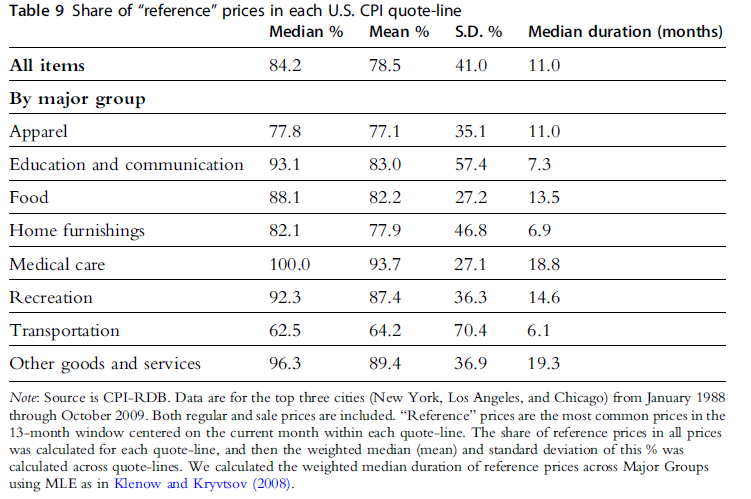
\includegraphics[trim=0 0 0 0,clip,width=0.7\textwidth]{FIGURES/PriceSetting/Table9_referencePrices}
	}      

\end{figure}
%\vspace{-2mm}

%\begin{minipage}{0.6\columnwidth}
%\tiny	
%%\textbf{Note.}
%\end{minipage}
\end{center}

\begin{itemize}
\small
\item $\rightarrow$ how much \tb{memory} is in prices?
\end{itemize}

\end{frame}
%---FRAME------------------------------------------------------------------------------
\begin{frame}{Comeback prices}

\begin{itemize}
\item \tb{Comeback price:} \emph{A price that appeared any time in the previous 12 months with a different price occurring at least once in between.}
\end{itemize}

\begin{center}
\begin{figure}[h!]
	\subfigure{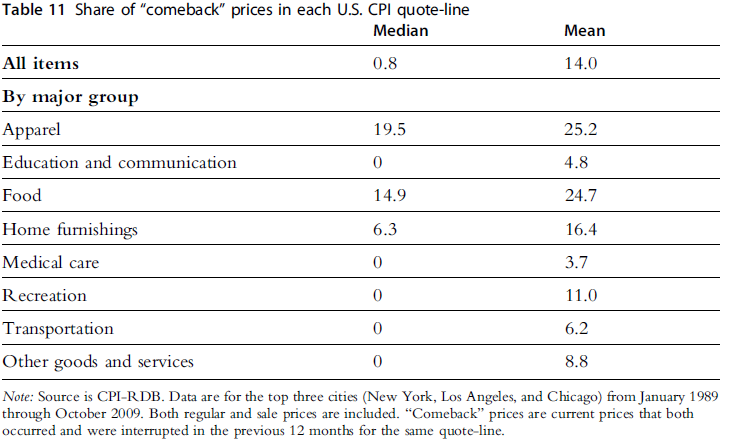
\includegraphics[trim=0 0 0 0,clip,width=0.7\textwidth]{FIGURES/PriceSetting/Table11_comebackPrices}
	}      

\end{figure}
%\vspace{-2mm}

%\begin{minipage}{0.6\columnwidth}
%\tiny	
%%\textbf{Note.}
%\end{minipage}
\end{center}

\begin{itemize}
\small
\item $\rightarrow$ Little memory in prices outside 'apparel' and 'food'
\end{itemize}

\end{frame}
%---FRAME------------------------------------------------------------------------------
\begin{frame}{Novel prices}

\begin{itemize}
\item \tb{Novel price:} \emph{A price that did not appear in any of the previous 12 months.}
\end{itemize}

\begin{center}
\begin{figure}[h!]
	\subfigure{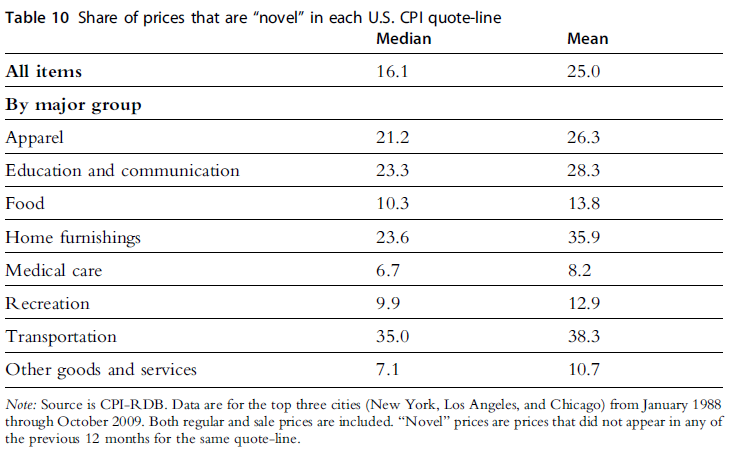
\includegraphics[trim=0 0 0 0,clip,width=0.7\textwidth]{FIGURES/PriceSetting/Table10_novelPrices}
	}      

\end{figure}
%\vspace{-2mm}

%\begin{minipage}{0.6\columnwidth}
%\tiny	
%%\textbf{Note.}
%\end{minipage}
\end{center}


\end{frame}
%---FRAME------------------------------------------------------------------------------
\section{10 Facts}
%---FRAME------------------------------------------------------------------------------
\begin{frame}{10 Facts - And Implications for Macro Models}

\begin{itemize}
\small
\item \tb{Fact 1:} Prices change at least once a year
\begin{itemize}
\small
\item Real effects of monetary policy lasting 3-5 years. Nominal rigidity alone cannot do the trick!
\end{itemize}
\item \tb{Fact 2:} Sales and product turnover are often important for micro price flexibility
\begin{itemize}
\small
\item Sales more important to micro level price flexibility, less macro level
\item ...but do not cancel out at the macro level, either.
\item e.g. United States with more sales than in the Euro Area
\end{itemize}
\item \tb{Fact 3:} Reference prices are stickier and more persistent than regular prices
\begin{itemize}
\small
\item closer to actual inflation
\end{itemize}
\item \tb{Fact 4:} There is substantial heterogeneity in the frequency of price change across goods
\item \tb{Fact 5:} More cyclical goods change prices more frequently
\begin{itemize}
\small
\item ...but question of causality unsettled.
\end{itemize}
\end{itemize}

\end{frame}
%---FRAME------------------------------------------------------------------------------
\begin{frame}{10 Facts - And Implications for Macro Models}

\begin{itemize}
\small
\item \tb{Fact 6:} Price changes are big on average, but many small changes occur
\begin{itemize}
\small
\item micro price jumps are an order of magnitude larger than the level of inflation: idiosyncratic forces dominate macro shocks
\end{itemize}
\item \tb{Fact 7:} Relative price changes are transitory
\item \tb{Fact 8:} Price changes are typically not synchronized over the business cycle
\begin{itemize}
\small
\item preoccupation with idiosyncratic over aggregate shocks (e.g. rational inattention)
\item more synchronization in times of larger macro volatility (Mexico)
\end{itemize}
\item \tb{Fact 9:} Neither frequency nor size is increasing in the age of a price
\begin{itemize}
\small
\item \emph{state-dependent pricing model} would imply higher hazard rate in the age of a price
\item \emph{time-dependent pricing model} would imply that the siye of price changes is increasing in the duration of stickiness
\end{itemize}
\item \tb{Fact 10:} Price changes are linked to wage changes
\begin{itemize}
\small
\item cross-sectional correlation between wage and price flexibility
\end{itemize}
\end{itemize}

\end{frame}
%---FRAME------------------------------------------------------------------------------
\section{Modeling nominal rigidities}
%---FRAME------------------------------------------------------------------------------
\begin{frame}
\frametitle{Outline}
\tableofcontents[currentsection]
\end{frame}
%---FRAME------------------------------------------------------------------------------

%---FRAME------------------------------------------------------------------------------
\begin{frame}{Modeling nominal rigidities}

\tb{Definition:} Nominal rigidity lead nominal wages and/or prices to adjust incompletely to changes in the nominal quantity of money.

\begin{itemize}
\small
\item State-dependent approaches:
\begin{itemize}
\item Menu cost (Rothenberg 1982)
\item Information frictions (Mankiw, Reis 2002)
\end{itemize}
\item Time-dependent approaches:
\begin{itemize}
\item Staggered contracts (Taylor 1980)
\item Stochastic price setting (Calvo 1983)
\end{itemize}
\end{itemize}

\end{frame}
%---FRAME------------------------------------------------------------------------------
\begin{frame}{State-dependent price setting}

\tb{Menu cost}
\begin{itemize}
\small
\item Imagine firm faces improved demand condition allowing for an extra profit of 1000 EUR
\item The cost of printing a new menu, however, is 2000 EUR
\item The restaurant will leave prices as they are.
\item Broader interpretation: cost of upsetting customers, adjustments to IT, ...
\end{itemize}

\tb{Information frictions}
\begin{itemize}
\small
\item Every period, only a fraction $\lambda$ of firms gathers information about the state of the economy
\item Remaining fraction of firms $(1-\lambda)$ does not update their prices.
\item Changes in the state of the economy only gradually translate into prices
\end{itemize}

\end{frame}
%---FRAME------------------------------------------------------------------------------
\begin{frame}{Time-dependent price setting}

\tb{Staggered contracts}
\begin{itemize}
\small
\item Firms can reset prices every $n^{th}$ period.
\item duration of the price spell is known
\item There are $n$ discrete price spell lengths
\end{itemize}

\tb{Stochastic price setting}
\begin{itemize}
\small
\item Firms face a constant probability $(1-\theta)$ to reset prices in period $t$.
\item A price will last for $i$ periods with probability $(\theta)^(i-1)$.
\item Expected duration of a price spell is $\frac{1}{(1-\theta)}$.
\item $\rightarrow$ a distribution with price spell lenghts
\end{itemize}


\end{frame}
%---FRAME------------------------------------------------------------------------------
\begin{frame}{Summary: Model features and the facts}


\begin{center}
\begin{figure}[h!]
	\subfigure{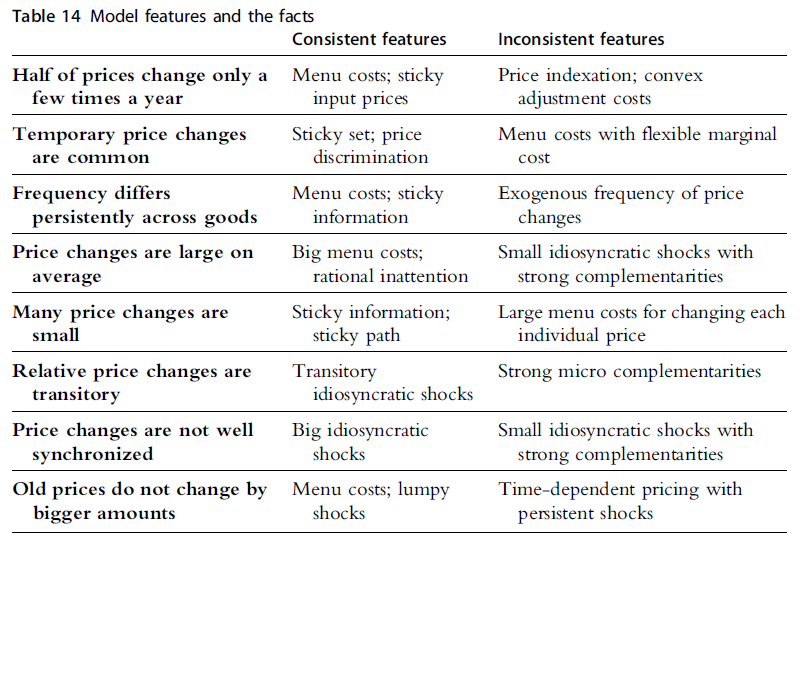
\includegraphics[trim=0 0 0 0,clip,width=1.0\textwidth]{FIGURES/PriceSetting/Table14_ModelFeaturesFacts}
	}      

\end{figure}
%\vspace{-2mm}

%\begin{minipage}{0.6\columnwidth}
%\tiny	
%%\textbf{Note.}
%\end{minipage}
\end{center}

\end{frame}
%---FRAME------------------------------------------------------------------------------
%---FRAME------------------------------------------------------------------------------
\begin{frame}{Summary:
 Nominal rigidities}

\emph{In this lecture...}

\begin{enumerate}
\item Reviewed empirical literature on price rigidities
\item Found that frequency of price changes is very heterogeneous; and this heterogeneity is not random
\item Discussed potential implications for macroeconomy
\item State discrepancies between data and modelling approaches 
\end{enumerate}

\emph{Next lecture:} sticky wages in the new Keynesian model (time-dependent Calvo-Yun pricing)

\end{frame}
%%---FRAME------------------------------------------------------------------------------
%---END------------------------------------------------------------------------------
\begin{frame}

\vspace{10mm}
\begin{center}
{\Large
\tb{Thank you.}\\
}
\vspace{10mm}
\footnotesize{
{\color{dblue}{\texttt{christoph.grossesteffen@banque-france.fr}}
}}
\end{center}

\end{frame}
%---END------------------------------------------------------------------------------
\end{document}

